\documentclass[10pt, aspectratio=43]{beamer}

\usepackage[polish]{babel}
\usepackage[utf8]{inputenc}
\usepackage[T1]{fontenc}
\usepackage{lmodern}
\usepackage{textcomp}

\usepackage{amsmath}
\usepackage{amssymb}
\usepackage{mathtools}
\usepackage{icomma}
\usepackage{graphicx}
\usepackage{caption}
\usepackage{subfigure}

\DeclareMathOperator{\arth}{arth}
\DeclareMathOperator{\sgn}{sgn}

\usetheme{Madrid}

\title[Dynamika z oporami]{Dynamika ruchu z oporami ośrodka}
\subtitle{Spadek swobodny i rzut ukośny -- ujęcie zaawansowane}
\author{Karol Peszek}
\institute{WFAIS}
\date{17 grudnia 2025}

\begin{document}

\begin{frame}
    \titlepage
\end{frame}

\begin{frame}{Plan wykładu}
    \tableofcontents
\end{frame}

\section{Wstęp i klasyfikacja oporów}

\begin{frame}{Rzeczywistość vs. Idealizacja}
    W dotychczasowych rozważaniach (np. rzut ukośny w próżni) zakładaliśmy, że jedyną siłą działającą na ciało jest siła grawitacji:
    \begin{equation}
        m\vec{a} = m\vec{g}
    \end{equation}
    W rzeczywistych ośrodkach płynnych (powietrze, woda, olej) na ciało działa siła oporu aerodynamicznego/hydrodynamicznego $\vec{F}_o$. Równanie ruchu (II zasada dynamiki Newtona) przyjmuje postać:
    \begin{equation}
        m\frac{d\vec{v}}{dt} = m\vec{g} + \vec{F}_o(\vec{v})
    \end{equation}
    Siła oporu $\vec{F}_o$ jest funkcją prędkości, kształtu ciała oraz parametrów ośrodka i jest zawsze skierowana przeciwnie do wektora prędkości chwilowej.
\end{frame}

\begin{frame}{Liczba Reynoldsa i reżimy przepływu}
    Kluczowym parametrem bezwymiarowym jest liczba Reynoldsa:
    \begin{equation}
        \mathrm{Re} = \frac{\rho v L}{\eta}
    \end{equation}
    gdzie: $\rho$ -- gęstość, $v$ -- prędkość, $L$ -- wymiar, $\eta$ -- lepkość.

    \textbf{Dwa główne reżimy oporu:}
    \begin{itemize}
        \item $\mathrm{Re} \ll 1$ (Laminarny/Stokesa): Dominują siły lepkości.
        \begin{itemize}
            \item \textbf{Model:} Opór liniowy $\vec{F}_o \propto -\vec{v}$.
            \item \textit{Przykłady:} Opadanie mgły, pył wulkaniczny, ruch bakterii.
        \end{itemize}
        \item $\mathrm{Re} \gg 1$ (Turbulentny/Newtona): Dominują siły bezwładności.
        \begin{itemize}
            \item \textbf{Model:} Opór kwadratowy $\vec{F}_o \propto -v\vec{v}$.
            \item \textit{Przykłady:} Samochody, samoloty, skoczek spadochronowy.
        \end{itemize}
    \end{itemize}

    \begin{alertblock}{Ważne}
        Model oporu liniowego jest przybliżeniem poprawnym wyłącznie dla $\mathrm{Re} \ll 1$ i traci sens fizyczny w przepływie turbulentnym. Oba modele są przybliżeniami, a nie prawami uniwersalnymi.
    \end{alertblock}
\end{frame}

\begin{frame}{Porównanie modeli oporu – zakresy i ograniczenia}
    \begin{table}
        \centering
        \small
        \begin{tabular}{|p{0.2\textwidth}|p{0.15\textwidth}|p{0.2\textwidth}|p{0.3\textwidth}|}
            \hline
            \textbf{Model oporu} & \textbf{Postać siły} & \textbf{Zakres Re} & \textbf{Ograniczenia} \\
            \hline
            Liniowy (Stokes) & $\vec{F} = -b\vec{v}$ & $\mathrm{Re} \ll 1$ & Niepoprawny dla dużych prędkości i obiektów makroskopowych. \\
            \hline
            Kwadratowy (Newton) & $\vec{F} = -cv\vec{v}$ & $10^3 < \mathrm{Re} < 10^5$ & Nie uwzględnia kryzysu oporu i efektów przyściennych przy bardzo małych v. \\
            \hline
        \end{tabular}
        \caption{Zestawienie modeli oporu aerodynamicznego.}
    \end{table}
\end{frame}

\section{Fizyka powstawania oporu}

\begin{frame}{Mechanizmy powstawania siły oporu}
    Całkowita siła oporu jest sumą dwóch składowych o różnej naturze fizycznej:
    
    \begin{enumerate}
        \item \textbf{Opór ciśnieniowy (kształtu):}
        Wynika z różnicy ciśnień między przednią a tylną częścią ciała.
        \begin{itemize}
            \item Przód: punkt spiętrzenia (nadciśnienie).
            \item Tył: oderwanie strugi i powstanie śladu aerodynamicznego (podciśnienie).
            \item Dominuje przy dużych $\mathrm{Re}$ (opór kwadratowy).
        \end{itemize}
        
        \item \textbf{Opór tarcia (lepkości):}
        Wynika z naprężeń stycznych w warstwie przyściennej płynu.
        \begin{itemize}
            \item Cząsteczki płynu "przyklejają się" do powierzchni ciała.
            \item Dominuje przy małych $\mathrm{Re}$ oraz dla ciał bardzo smukłych.
        \end{itemize}
    \end{enumerate}
\end{frame}

\begin{frame}{Kryzys oporu (Drag Crisis)}
    Dla kuli, przy $\mathrm{Re} \approx 3 \cdot 10^5$, obserwujemy gwałtowny spadek współczynnika oporu $C_x$ (z $0,5$ do $0,1$).
    
    \textbf{Mechanizm fizyczny:}
    \begin{itemize}
        \item Przejście warstwy przyściennej z laminarnej w turbulentną.
        \item Warstwa turbulentna ma większą energię kinetyczną przy powierzchni, co pozwala jej dłużej przylegać do opływanego ciała.
        \item \textbf{Efekt:} Punkt oderwania strugi przesuwa się do tyłu $\rightarrow$ węższy ślad aerodynamiczny $\rightarrow$ mniejszy opór ciśnieniowy.
    \end{itemize}
    
    \textit{Przykład: Dołeczki na piłeczce golfowej wymuszają turbulencję warstwy przyściennej, zmniejszając opór i zwiększając zasięg.}
\end{frame}

\begin{frame}{Opór indukowany}
    Występuje wyłącznie dla ciał generujących siłę nośną (np. skrzydła o skończonej rozpiętości).
    
    \begin{itemize}
        \item Wynika z wyrównywania ciśnień na końcach płata (przepływ z dołu na górę).
        \item Powstają wiry brzegowe, które zmieniają efektywny kąt natarcia i odchylają wektor siły aerodynamicznej do tyłu.
        \item Jest odwrotnie proporcjonalny do wydłużenia skrzydła i prędkości ($F_{ind} \sim 1/v^2$).
    \end{itemize}
        \begin{figure}
        \centering
        \begin{columns}
            \column{0.5\textwidth}
            \centering
            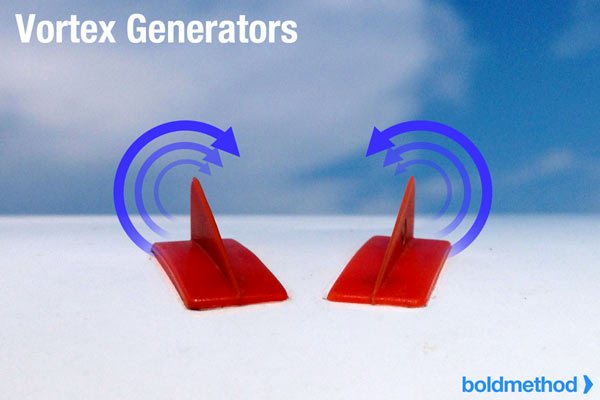
\includegraphics[width=0.95\linewidth, height=3.5cm, keepaspectratio]{vortex.jpg}
            \caption{Wiry}
            \column{0.5\textwidth}
            \centering
            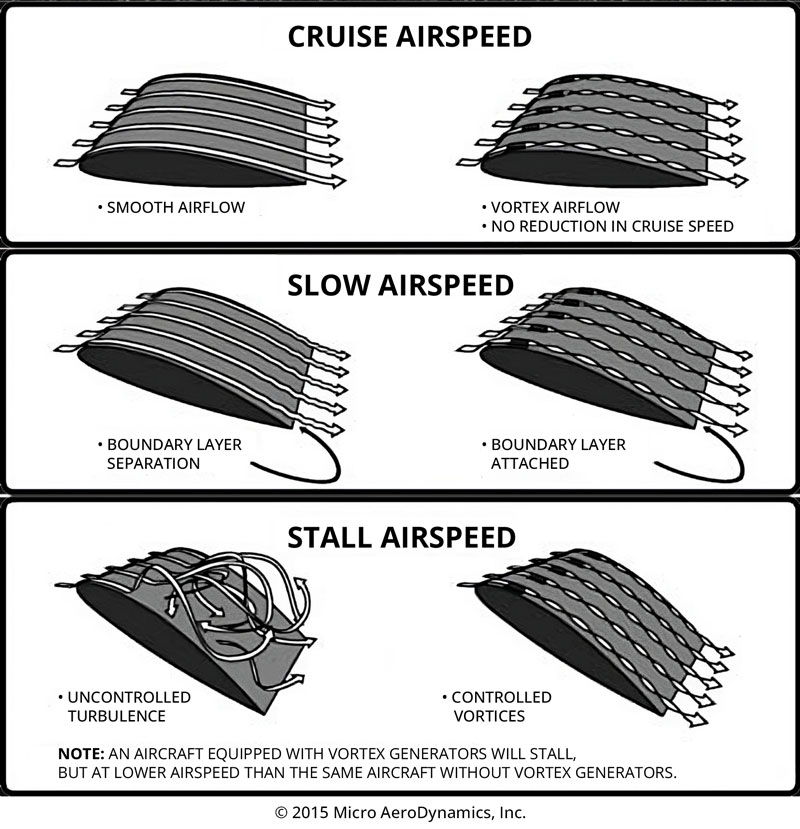
\includegraphics[width=0.95\linewidth, height=3.5cm, keepaspectratio]{wings.jpg}
            \caption{Skrzydła}
        \end{columns}
    \end{figure}
\end{frame}

\section{Model I: Opór Liniowy (Prawo Stokesa)}

\begin{frame}{Opór Liniowy - Równania ruchu}
    Dla małych prędkości ($\vec{F}_o = -b\vec{v}$). Rozważmy rzut ukośny.
    Układ współrzędnych: Oś Y skierowana w górę, grawitacja w dół.
    
    Równanie wektorowe: $m\dot{\vec{v}} = m\vec{g} - b\vec{v}$.
    
    Rozkład na składowe (separacja zmiennych jest możliwa!):
    \begin{align}
        \text{Oś X:} \quad & m\dot{v}_x = -b v_x \\
        \text{Oś Y:} \quad & m\dot{v}_y = -mg - b v_y
    \end{align}
    
    Zdefiniujmy stałą czasową relaksacji: $\tau = \frac{m}{b}$.
\end{frame}

\begin{frame}{Oś X: Wyprowadzenie analityczne}
    Rozwiązujemy równanie jednorodne dla składowej poziomej:
    \begin{equation}
        \frac{dv_x}{dt} = -\frac{b}{m} v_x = -\frac{1}{\tau} v_x
    \end{equation}
    Rozdzielamy zmienne i całkujemy:
    \begin{equation}
        \int_{v_{0x}}^{v_x(t)} \frac{dv'_x}{v'_x} = -\frac{1}{\tau} \int_0^t dt'
    \end{equation}
    \begin{equation}
        \ln \left( \frac{v_x(t)}{v_{0x}} \right) = -\frac{t}{\tau} \implies \boxed{v_x(t) = v_{0x} e^{-\frac{t}{\tau}}}
    \end{equation}
    Położenie $x(t)$:
    \begin{equation}
        x(t) = \int_0^t v_x(t') dt' = v_{0x} \tau \left( 1 - e^{-\frac{t}{\tau}} \right)
    \end{equation}
    \textit{Wniosek: Zasięg w poziomie jest skończony i wynosi $x_{max} = v_{0x}\tau$.}
\end{frame}

\begin{frame}{Oś Y: Spadek i wznoszenie}
    Równanie dla osi pionowej (niejednorodne):
    \begin{equation}
        \dot{v}_y + \frac{1}{\tau}v_y = -g
    \end{equation}
    Rozwiązanie ogólne to suma rozwiązania jednorodnego ($Ce^{-t/\tau}$) i szczególnego ($-g\tau$).
    Niech $v_{gr} = g\tau = \frac{mg}{b}$ (wartość dodatnia). Wtedy asymptotą jest $-v_{gr}$.
    
    Rozwiązanie dla warunku początkowego $v_y(0) = v_{0y}$:
    \begin{equation}
        \boxed{v_y(t) = (v_{0y} + v_{gr})e^{-\frac{t}{\tau}} - v_{gr}}
    \end{equation}
    
    Położenie $y(t)$:
    \begin{equation}
        y(t) = (v_{0y} + v_{gr})\tau (1 - e^{-\frac{t}{\tau}}) - v_{gr}t + y_0
    \end{equation}
\end{frame}

\begin{frame}{Wykresy ruchu z oporem liniowym}
    \begin{figure}
        \centering
        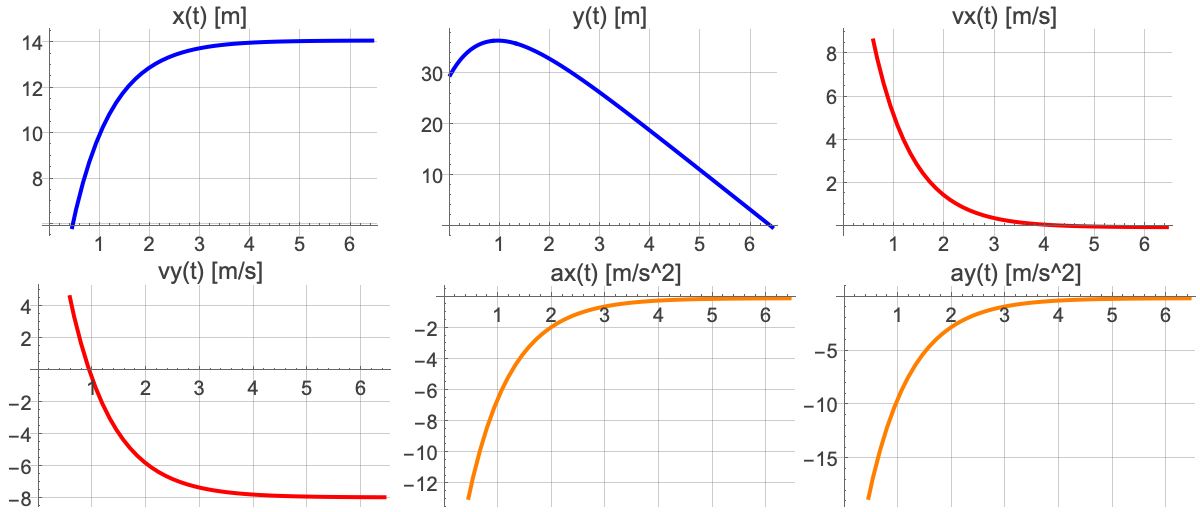
\includegraphics[width=\linewidth, height=5cm, keepaspectratio]{lin_plot.png}
        \caption{Przykładowe wykresy prędkości i położenia dla rzutu ukośnego z oporem liniowym.}
    \end{figure}
\end{frame}

\section{Model II: Opór Kwadratowy (Turbulentny)}

\begin{frame}{Opór kwadratowy}
    W przepływie turbulentnym siła oporu zależy od kwadratu prędkości.
    \alert{Uwaga na zapis wektorowy!} Nie możemy napisać $\vec{F}_o \sim v^2$, bo to skalar.
    
    Poprawny zapis siły oporu:
    \begin{equation}
        \vec{F}_o = -\frac{1}{2} C_x \rho S |\vec{v}| \vec{v}
    \end{equation}
    lub krócej, wprowadzając stałą $c = \frac{1}{2} C_x \rho S$:
    \begin{equation}
        \vec{F}_o = -c v \vec{v} \quad (\text{gdzie } v = |\vec{v}|)
    \end{equation}
    
    Siła jest przeciwna do wektora prędkości, a jej wartość to $F_o = c v^2$.
\end{frame}

\begin{frame}{Spadek swobodny (1D) - Rozwiązanie}
    Dla spadku pionowego ($v_x=0, v_y=v$), równanie ruchu przyjmuje postać skalarną:
    \begin{equation}
        m\dot{v} = mg - cv^2 \implies \dot{v} = g \left( 1 - \frac{v^2}{v_{gr}^2} \right)
    \end{equation}
    gdzie $v_{gr} = \sqrt{\frac{mg}{c}}$. Całkujemy:
    \begin{equation}
        \int \frac{dv}{1 - (v/v_{gr})^2} = g \int dt \implies v_{gr} \arth\left(\frac{v}{v_{gr}}\right) = gt
    \end{equation}
    Ostatecznie:
    \begin{equation}
        \boxed{v(t) = v_{gr} \tanh\left( \frac{gt}{v_{gr}} \right)}
    \end{equation}
\end{frame}

\begin{frame}{Rzut ukośny z oporem kwadratowym - Sprzężenie}
    Rozpiszmy równanie wektorowe na składowe. Pamiętając, że $|\vec{v}| = \sqrt{v_x^2 + v_y^2}$:
    
    \begin{align}
        m\ddot{x} &= -c \left( \sqrt{\dot{x}^2 + \dot{y}^2} \right) \dot{x} \\
        m\ddot{y} &= -mg - c \left( \sqrt{\dot{x}^2 + \dot{y}^2} \right) \dot{y}
    \end{align}
    
    \textbf{Problem analityczny:}
    Równania są \textbf{silnie sprzężone}. W równaniu na $x$ występuje $\dot{y}$, a w równaniu na $y$ występuje $\dot{x}$.
    \begin{itemize}
        \item Brak ścisłego rozwiązania analitycznego w postaci zamkniętej.
        \item Konieczność stosowania metod numerycznych.
        \item Tor lotu nie jest parabolą, lecz krzywą balistyczną z pionową asymptotą.
    \end{itemize}
\end{frame}

\begin{frame}{Wykresy ruchu z oporem kwadratowym}
    \begin{figure}
        \centering
        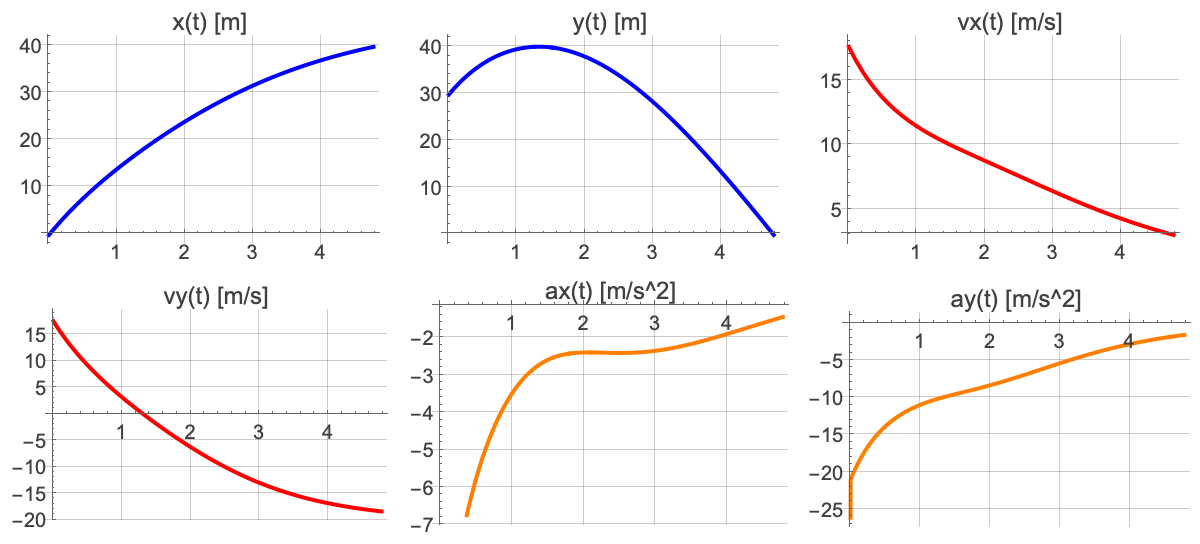
\includegraphics[width=\linewidth, height=5cm, keepaspectratio]{quad_plot.png}
        \caption{Przykładowe wykresy prędkości i położenia dla rzutu ukośnego z oporem liniowym.}
    \end{figure}
\end{frame}

\section{Współczynniki aerodynamiczne w praktyce}

\begin{frame}{Wartości współczynnika $C_x$ (Drag Coefficient)}
    Współczynnik $C_x$ jest miarą "doskonałości aerodynamicznej" kształtu.
    
    \begin{table}
        \centering
        \begin{tabular}{l|c|l}
            \textbf{Obiekt} & \textbf{$C_x$} & \textbf{Komentarz} \\
            \hline
            Płyta prostopadła & $\approx 1,28$ & Dominujący opór ciśnieniowy \\
            Sześcian & $\approx 1,05$ & \\
            Autobus & $\approx 0,70$ & Pudełkowaty kształt \\
            Kula & $0,47$ & Przepływ laminarny \\
            \textbf{Fiat 126p} & $\mathbf{0,47}$ & "Maluch" ma aerodynamikę kuli \\
            Samochód osobowy & $0,30 - 0,35$ & Typowy sedan \\
            \textbf{Tesla Model S} & $\mathbf{0,24}$ & Nowoczesna optymalizacja \\
            Profil lotniczy & $0,04$ & Kształt kroplowy, minimalizacja oderwania \\
        \end{tabular}
        \caption{Przykładowe wartości współczynnika oporu.}
    \end{table}
\end{frame}

\section{Podsumowanie i Zadania}

\begin{frame}{Zadanie domowe}
    \textbf{Problem do samodzielnego rozwiązania:}
    
    Rozważmy rzut ukośny z oporem liniowym. Wyprowadziliśmy wzory na $x(t)$ i $y(t)$.
    Wykaż, stosując rozwinięcie w szereg Taylora funkcji $e^{-x} \approx 1 - x + \frac{x^2}{2}$, że dla bardzo krótkich czasów ($t \ll \tau$) równania ruchu redukują się do klasycznych równań rzutu w próżni (parabola).
    
    \vspace{1cm}
    \centering
    \textit{Dziękuję za uwagę.}
\end{frame}

\begin{frame}{Literatura}
    \begin{thebibliography}{9}
        \bibitem{landau}
        L.D. Landau, E.M. Lifshitz,
        \textit{Hydrodynamika. Fizyka teoretyczna. Tom 6},
        Wydawnictwo Naukowe PWN.
        
        \bibitem{feynman}
        R.P. Feynman, R.B. Leighton, M. Sands,
        \textit{Feynmana wykłady z fizyki. Tom 2},
        Wydawnictwo Naukowe PWN.

        \bibitem{resnick}
        D. Halliday, R. Resnick, J. Walker,
        \textit{Podstawy fizyki},
        Wydawnictwo Naukowe PWN.

        \bibitem{wiki}
        Wikipedia,
        \textit{Opór aerodynamiczny},
        \url{https://en.wikipedia.org/wiki/Drag_(physics)}.
    \end{thebibliography}
\end{frame}

\end{document}


